\chapter{Análisis del Sistema}

\section{Análisis de Requerimientos}

En esta sección se describen los requerimientos funcionales y no funcionales del sistema propuesto, los cuales establecen las capacidades, restricciones y criterios de desempeño que debe cumplir la solución desarrollada. Estos requerimientos sirven como base para el diseño, implementación y evaluación del sistema, asegurando la trazabilidad entre las necesidades del evaluador y la arquitectura final.

% =========================================================
\subsection{Requerimientos Funcionales}
% =========================================================

Los requerimientos funcionales definen las capacidades y procesos que el sistema debe implementar para cumplir con las funciones de análisis, gestión de información y auditoría de código en el contexto académico.

\begin{itemize}
    \item \textbf{RF-01:} El sistema debe permitir el registro e inicio de sesión de docentes mediante credenciales cifradas para garantizar un espacio de trabajo privado.
    
    \item \textbf{RF-02:} El sistema debe permitir al docente la creación y gestión de un listado de ejercicios o problemas de programación (Biblioteca).
    
    \item \textbf{RF-03:} El sistema debe permitir la carga de código fuente en formato .c y .cpp asociados a un ejercicio específico.
    
    \item \textbf{RF-04:} El sistema debe realizar el preprocesamiento y normalización del código fuente, asegurando la correcta extracción de los grafos para el canal semántico, mientras se preserva la integridad de las estructuras de estilo originales para el detección de patrones generativos.
    
    \item \textbf{RF-05:} El sistema debe generar representaciones basadas en Grafos de Flujo de Datos (DFG) para el módulo semántico, y transformar el código fuente en secuencias matriciales bidimensionales (carácter por vector) para su procesamiento mediante convoluciones 1D en el módulo estilométrico.
    
    \item \textbf{RF-06:} El sistema debe realizar el análisis de similitud semántica mediante el modelo GraphCodeBERT para la generación de vectores de características (embeddings), cuantificando la proximidad entre ellos utilizando la métrica de similitud del coseno.
    
    \item \textbf{RF-07:} El sistema debe realizar el análisis estilométrico mediante el modelo CharCNN para calcular la probabilidad de generación mediante inteligencia artificial. sintética o humana.
    
    \item \textbf{RF-08:} El sistema debe solicitar y recibir múltiples versiones funcionalmente equivalentes del problema proporcionado por el docente a través de un modelo LLM externo.
    
    \item \textbf{RF-09:} El sistema debe realizar el almacenamiento persistente de los resultados del análisis y metadatos en una base de datos relacional (PostgreSQL), así como de los vectores de características en una base de datos vectorial (ChromaDB), asegurando la integridad referencial.
    
    \item \textbf{RF-10:} El sistema debe generar un reporte consolidado que integre el índice de similitud semántica y la probabilidad de generación mediante inteligencia artificial. de forma visual.
    
    \item \textbf{RF-11:} El sistema debe realizar una fusión de características (Feature Fusion) que integre el vector semántico y la probabilidad estilométrica, consolidando las métricas de ambos módulos en una sola estructura para su análisis dual.
    
    \item \textbf{RF-12:} El sistema debe permitir la consulta histórica de reportes de análisis realizados previamente sin necesidad de re-procesar los archivos fuente.
\end{itemize}

% =========================================================
\subsection{Requerimientos No Funcionales}
% =========================================================

Los requerimientos no funcionales establecen las restricciones, atributos de calidad y condiciones de desempeño que debe cumplir el sistema propuesto durante su operación.

\begin{itemize}
    \item \textbf{RNF-01:} Seguridad de datos: El sistema debe cifrar las contraseñas de los usuarios y utilizar tokens de sesión (JWT) para proteger la comunicación entre el cliente y el servidor.
    
    \item \textbf{RNF-02:} Persistencia híbrida: El sistema debe operar bajo un esquema de base de datos dual, optimizando las consultas relacionales en PostgreSQL y las búsquedas por similitud vectorial en ChromaDB.
    
    \item \textbf{RNF-03:} Los modelos de IA integrados deben estar calibrados buscando alcanzar un objetivo de rendimiento base de F1-Score $\ge$ 0.85 para GraphCodeBERT en tareas de detección de similitud semántica.
    
    \item \textbf{RNF-04:} El módulo estilométrico (CharCNN) debe estar optimizado para buscar una precisión de clasificación de autoría igual o superior a 0.8 bajo el corpus de pruebas establecido.
    
    \item \textbf{RNF-05:} El sistema debe soportar el análisis de código bajo los estándares C11 y C++17 para garantizar compatibilidad operativa con el currículo y las entregas esperadas.
    
    \item \textbf{RNF-06:} El orquestador de métricas debe ajustar los umbrales de decisión con el objetivo de mantener una tasa de falsos positivos menor al 10\% durante el análisis de doble canal.
    
    \item \textbf{RNF-07:} El tiempo de procesamiento de inferencia en el backend durante la fase de análisis de una entrega estudiantil no debe exceder los 20 segundos, dado que la indexación de referencias y la generación de variantes (LLM) se realizan de forma asíncrona en la fase de configuración previa.
    
    \item \textbf{RNF-08:} El sistema debe ser compatible para su ejecución en navegadores web basados en el motor Chromium versión 110 o superior.
    
    \item \textbf{RNF-09:} La interfaz web debe ser intuitiva, permitiendo ejecutar todas las tareas en 3 o menos acciones y proporcionar retroalimentación visual o indicadores de estado en tiempo real mientras el orquestador (LangGraph) procesa las tareas en segundo plano.
    
    \item \textbf{RNF-10:} El sistema debe asegurar alta disponibilidad operativa durante el procesamiento y análisis de código dentro del entorno de despliegue asignado para las pruebas.
    
    \item \textbf{RNF-11:} El sistema debe realizar validaciones preventivas en el cliente (tipo de archivo, tamaño e integridad) antes de iniciar la transmisión de la carga útil hacia la API REST.
\end{itemize}

% =========================================================
\subsection{Reglas de Negocio}
% =========================================================

Las reglas de negocio definen los criterios que guían el funcionamiento y uso ético del sistema dentro del entorno académico.

\begin{itemize}
    \item \textbf{RN-01:} Confidencialidad de los datos: Un docente solo podrá visualizar, editar y consultar los ejercicios y reportes generados bajo su propia cuenta de usuario.
    
    \item \textbf{RN-02:} El sistema se limita a programas de cursos de programación de ESCOM-IPN que sigan los estándares C11 y C++17.
    
    \item \textbf{RN-03:} Integridad de la referencia: Toda entrega debe ser comparada contra al menos una solución de referencia proporcionada por el docente para ser considerada válida.
    
    \item \textbf{RN-04:} La decisión final de calificación es responsabilidad exclusiva del docente; el sistema actúa únicamente como una herramienta objetiva de apoyo a la auditoría académica.
    
    \item \textbf{RN-05:} Se permite el uso de múltiples soluciones generadas por LLM para ampliar el espectro de comparación lógica, siempre que el docente las valide inicialmente.
    
    \item \textbf{RN-06:} Preservación de referencias: Los archivos cargados en calidad de entregas a analizar no podrán ser catalogados ni reutilizados por el sistema como códigos de referencia para futuras comparaciones, garantizando que el estándar de comparación se mantenga basado exclusivamente en soluciones validadas o generadas por el docente.
\end{itemize}

% =========================================================
\section{Identificación y descripción de actores}
% =========================================================

En el contexto del sistema propuesto (Graphito), los actores representan las entidades externas que interactúan con la plataforma y que participan en el flujo de configuración, análisis y auditoría del código fuente. La correcta identificación de estos actores permite definir los casos de uso, delimitar responsabilidades y establecer las fronteras del sistema.

A partir de la arquitectura funcional, se identifican exclusivamente dos actores que interactúan de forma directa con la plataforma:

% ---------------------------------------------------------
\subsection{Docente / Evaluador}
% ---------------------------------------------------------

Es el actor principal y humano del sistema. Utiliza la plataforma como una herramienta de apoyo a la decisión en su proceso de auditoría académica (correspondiente a profesores o instructores de programación).

Entre sus principales responsabilidades de interacción se encuentran:

\begin{itemize}
    \item Proporcionar la descripción técnica del problema o práctica.
    \item Configurar el marco de comparación cargando sus códigos de referencia.
    \item Cargar los archivos fuente (\textit{.c, .cpp}) desarrollados por los estudiantes para su análisis.
    \item Interpretar los reportes visuales generados por el sistema, incluyendo los índices de similitud semántica y la probabilidad de generación mediante inteligencia artificial..
    \item Tomar la decisión final sobre la calificación del alumno, utilizando la evidencia estática proporcionada por la herramienta.
\end{itemize}

% ---------------------------------------------------------
\subsection{Motor de Inteligencia Artificial Externo (LLM)}
% ---------------------------------------------------------

Este actor corresponde a una API de un sistema externo basado en Modelos de Lenguaje Grande (LLM). Actúa como un proveedor de servicios de generación de código sintético bajo demanda.

Sus funciones en interacción con el orquestador de Graphito son:

\begin{itemize}
    \item Recibir el código de referencia original y generar descripciones técnicas algorítmicas.
    \item Generar múltiples variantes de código que sean funcionalmente equivalentes a la referencia del docente.
    \item Proveer el insumo necesario para que el sistema indexe un espacio vectorial de comparación mucho más robusto.
\end{itemize}

% =========================================================
\section{Trayectorias principales y alternativas}
% =========================================================

Las trayectorias describen el flujo de interacción entre el docente, el orquestador backend y los modelos de IA, detallando las secuencias de acciones para llevar a cabo el análisis bimodal. Estas trayectorias reflejan el comportamiento esperado (Modelado BPMN) y los escenarios alternativos.

% ---------------------------------------------------------
\subsection{Trayectoria principal (Flujo de Análisis Estándar)}
% ---------------------------------------------------------

La trayectoria principal describe el flujo de uso del sistema para procesar una entrega estudiantil contra referencias previamente configuradas.

\begin{enumerate}
    \item El docente accede a su biblioteca en la plataforma web del sistema.
    \item El docente carga el archivo fuente a analizar, seleccionando el problema correspondiente.
    \item El backend recibe el código y ejecuta el preprocesamiento y normalización (limpieza para el canal semántico y preservación de formato para el estilométrico).
    \item \textbf{Canal Semántico:} Se extrae el Grafo de Flujo de Datos (DFG) y el modelo \textit{GraphCodeBERT} genera el embedding estructural.
    \item \textbf{Canal Estilométrico:} El modelo \textit{CharCNN} procesa la matriz de caracteres 1D para estimar la probabilidad de generación mediante inteligencia artificial.
    \item El orquestador ejecuta la \textbf{Fusión de Características (Feature Fusion)} unificando ambos resultados.
    \item El sistema calcula la similitud del coseno del vector unificado contra la base de datos vectorial (\textit{ChromaDB}).
    \item El sistema consolida los resultados y persiste los metadatos en la base de datos relacional (\textit{PostgreSQL}).
    \item El sistema renderiza el reporte de análisis dual.
    \item El docente visualiza los indicadores numéricos y toma una decisión informada.
\end{enumerate}

% ---------------------------------------------------------
\subsection{Trayectorias alternativas}
% ---------------------------------------------------------

Las trayectorias alternativas describen variaciones del flujo principal, orquestadas por \textit{LangGraph} ante condiciones específicas.

\textbf{A1. Robustecimiento de referencias mediante LLM}

\begin{enumerate}
    \item Durante la configuración de un problema, el docente solicita la generación de variantes de su solución.
    \item El sistema envía el código de referencia al LLM externo.
    \item El modelo externo retorna múltiples soluciones equivalentes.
    \item El sistema calcula los embeddings semánticos de estas variantes y los indexa en la base vectorial de forma asíncrona.
\end{enumerate}

\textbf{A2. Código con errores críticos de formato}

\begin{enumerate}
    \item El sistema detecta inconsistencias irreparables durante la normalización inicial del código.
    \item El orquestador detiene el flujo antes de la inferencia de los modelos.
    \item Se notifica al docente en la interfaz sobre la invalidez del archivo fuente.
\end{enumerate}

\textbf{A3. Análisis estilométrico de baja confianza}

\begin{enumerate}
    \item El sistema identifica que el código cargado carece de una extensión mínima para extraer patrones de caracteres viables.
    \item El orquestador reduce la ponderación del canal estilométrico en la fusión de características.
    \item El sistema prioriza el índice de similitud semántica y añade una nota técnica en el reporte final.
\end{enumerate}

\textbf{A4. Alta equivalencia lógica detectada}

\begin{enumerate}
    \item El cálculo de la similitud del coseno arroja un valor superior al umbral establecido.
    \item El sistema clasifica la entrega como de alto interés de auditoría.
    \item Se destaca visualmente el registro en el panel del docente para sugerir una revisión prioritaria.
\end{enumerate}

\textbf{A5. Discrepancia crítica en análisis de doble canal}

\begin{enumerate}
    \item El orquestador detecta una correlación anómala (ej. alta similitud lógica combinada con una huella de autoría clasificada como inteligencia artificial).
    \item El sistema estructura un indicador visual de inconsistencia en el reporte final.
    \item El docente analiza el reporte detallado para auditar la anomalía.
\end{enumerate}

\section{Diagrama de Casos de Uso}

El análisis de casos de uso define las fronteras del sistema Graphito y describe las interacciones entre los actores externos y las funcionalidades internas. Este modelo permite visualizar cómo el evaluador gestiona el proceso de auditoría académica, desde la configuración inicial hasta la toma de decisiones basada en el reporte bimodal.

En la Figura~\ref{fig:casos_uso} se presenta el diagrama de casos de uso general del sistema, estructurado de forma jerárquica para reflejar el flujo de trabajo del docente.

\begin{figure}[H]
    \centering
    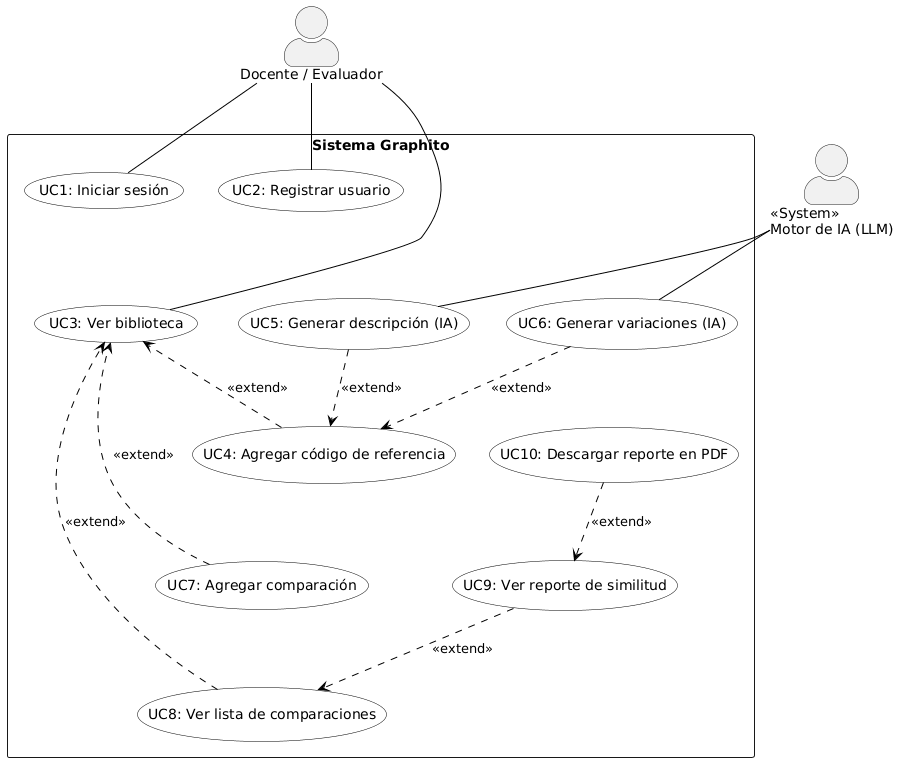
\includegraphics[width=0.75\textwidth]{figuras/casos_uso_v2.png} 
    \caption{Diagrama de casos de uso del sistema Graphito.}
    \label{fig:casos_uso}
\end{figure}

\subsection{Descripción de Actores}

Para el funcionamiento del sistema se han identificado dos actores principales:

\begin{itemize}
    \item \textbf{Docente / Evaluador:} Actor principal humano que interactúa con la plataforma para configurar problemas, gestionar entregas y visualizar los reportes de similitud.
    \item \textbf{Modelo LLM Externo:} Actor de sistema que actúa como proveedor de servicios de generación de código. Es consultado de forma opcional para robustecer el conjunto de referencias.
\end{itemize}

\subsection{Descripción de los Casos de Uso}

A continuación, se describen los módulos funcionales que integran la solución \textit{Graphito}, estructurados de acuerdo con su rol en el flujo de auditoría académica:

\begin{itemize}
    \item \textbf{Gestión de Acceso y Biblioteca (UC1, UC2, UC3):} Facilitan la administración de la sesión del docente y el acceso a la pagina principal (Biblioteca). Este módulo centraliza los ejercicios históricos y las comparaciones realizadas, permitiendo un entorno de trabajo persistente.
    \item \textbf{Gestión de Referencias y Pre-procesamiento (UC4, UC5, UC6, UC11):} Permiten al evaluador establecer el marco de comparación. Incluye la carga de soluciones base (UC4) y su enriquecimiento mediante un motor de IA externo para generar descripciones y variantes sintéticas (UC5, UC6). De forma obligatoria (\textit{include}), el sistema realiza la generación de \textit{embeddings} semánticos (UC11) sobre estas referencias.
    \item \textbf{Ejecución de Comparaciones (UC7, UC12):} Constituye el núcleo operativo del sistema. Al agregar una entrega para comparar (UC7), el sistema ejecuta automáticamente (\textit{include}) el análisis de doble canal (UC12), el cual integra el procesamiento semántico de flujo de datos y el detección de patrones generativos estilométrica.
    \item \textbf{Resultados y Reporteo (UC8, UC9, UC10):} Proporcionan la interfaz de auditoría donde se listan las comparaciones (UC8) y se visualizan los reportes de similitud detallados (UC9). Finalmente, se permite la exportación de resultados en formato PDF (UC10) para su integración en actas de evaluación.
\end{itemize}

\subsection{Especificación de Casos de Uso}

A continuación se detallan los casos de uso que rigen el comportamiento del sistema Graphito. Estas especificaciones describen la interacción detallada entre los actores y los módulos de inteligencia artificial.

% =========================================================
% ESPECIFICACIÓN DE CASOS DE USO
% =========================================================

% --- CASO DE USO 1 ---
\begin{table}[H]
\centering
\begin{tabular}{|p{3cm}|p{11cm}|}
\hline
\rowcolor[HTML]{E7F3FF} 
\textbf{Caso de Uso:} & \textbf{UC1: Iniciar sesión} \\ \hline
\textbf{Actor:} & Docente / Evaluador \\ \hline
\textbf{Descripción:} & El docente ingresa sus credenciales de acceso para entrar al sistema Graphito. \\ \hline
\textbf{Precondiciones:} & El docente debe estar registrado previamente en la plataforma (UC2). \\ \hline
\textbf{Flujo Básico:} & 
1. El docente ingresa su correo electrónico y contraseña en la interfaz. \newline
2. El sistema valida las credenciales mediante un proceso de autenticación cifrada contra la base de datos relacional (PostgreSQL). \newline
3. El sistema genera un token de sesión (JWT) y redirige al docente a su Biblioteca (UC3). \\ \hline
\textbf{Trayectorias Alternativas:} & Si las credenciales son incorrectas, el sistema muestra un mensaje de error y deniega el acceso, manteniendo la sesión cerrada. \\ \hline
\end{tabular}
\caption{Especificación del Caso de Uso 1.}
\end{table}

% --- CASO DE USO 2 ---
\begin{table}[H]
\centering
\begin{tabular}{|p{3cm}|p{11cm}|}
\hline
\rowcolor[HTML]{E7F3FF} 
\textbf{Caso de Uso:} & \textbf{UC2: Registrar usuario} \\ \hline
\textbf{Actor:} & Docente / Evaluador \\ \hline
\textbf{Descripción:} & Un nuevo docente crea una cuenta en la plataforma para poder gestionar sus ejercicios, referencias y comparaciones. \\ \hline
\textbf{Flujo Básico:} & 
1. El docente proporciona su nombre, correo electrónico y define una contraseña. \newline
2. El sistema cifra la contraseña y registra al nuevo usuario en PostgreSQL. \newline
3. El sistema confirma el registro exitoso y redirige a la vista de inicio de sesión. \\ \hline
\textbf{Postcondición:} & Se inicializa un espacio aislado en la base de datos para el repositorio personal del docente. \\ \hline
\end{tabular}
\caption{Especificación del Caso de Uso 2.}
\end{table}

% --- CASO DE USO 3 ---
\begin{table}[H]
\centering
\begin{tabular}{|p{3cm}|p{11cm}|}
\hline
\rowcolor[HTML]{E7F3FF} 
\textbf{Caso de Uso:} & \textbf{UC3: Ver biblioteca} \\ \hline
\textbf{Actor:} & Docente / Evaluador \\ \hline
\textbf{Descripción:} & Página principal del sistema donde el docente accede a su biblioteca personal, desde donde visualiza los problemas configurados previamente o inicia nuevas configuraciones. \\ \hline
\textbf{Precondiciones:} & El docente debe haber iniciado sesión de forma exitosa (UC1). \\ \hline
\textbf{Flujo Básico:} & 
1. El docente selecciona la opción de "Biblioteca" en la interfaz. \newline
2. El sistema recupera de PostgreSQL la lista de ejercicios asociados al identificador del docente. \newline
3. El sistema muestra la lista de ejercicios, habilitando las opciones de gestión (agregar referencia, ver comparaciones). \\ \hline
\textbf{Postcondición:} & El sistema queda a la espera de la ejecución de una acción extendida (UC4, UC7, UC8). \\ \hline
\end{tabular}
\caption{Especificación del Caso de Uso 3.}
\end{table}

% --- CASO DE USO 4 ---
\begin{table}[H]
\centering
\begin{tabular}{|p{3cm}|p{11cm}|}
\hline
\rowcolor[HTML]{E7F3FF} 
\textbf{Caso de Uso:} & \textbf{UC4: Agregar código de referencia} \\ \hline
\textbf{Actor:} & Docente / Evaluador \\ \hline
\textbf{Descripción:} & El docente carga el código fuente que servirá como solución ideal, inicializando el proceso asíncrono de indexación semántica. \\ \hline
\textbf{Precondiciones:} & El docente debe encontrarse gestionando un ejercicio dentro de la Biblioteca (UC3). \\ \hline
\textbf{Flujo Básico:} & 
1. El docente selecciona agregar una nueva referencia y carga el archivo (.c o .cpp). \newline
2. El sistema normaliza el código eliminando comentarios. \newline
3. El orquestador extrae el Grafo de Flujo de Datos (DFG) y genera el embedding correspondiente mediante GraphCodeBERT. \newline
4. El vector semántico resultante se almacena en ChromaDB. \newline
5. El sistema habilita las opciones para enriquecer la referencia utilizando un modelo de IA externo (UC5, UC6). \\ \hline
\textbf{Postcondición:} & El código base queda indexado en la base vectorial, preparado para futuras comparaciones. \\ \hline
\end{tabular}
\caption{Especificación del Caso de Uso 4.}
\end{table}

% --- CASO DE USO 5 ---
\begin{table}[H]
\centering
\begin{tabular}{|p{3cm}|p{11cm}|}
\hline
\rowcolor[HTML]{E7F3FF} 
\textbf{Caso de Uso:} & \textbf{UC5: Generar descripción (IA)} \\ \hline
\textbf{Actor:} & Motor de IA (LLM) / Docente \\ \hline
\textbf{Descripción:} & El sistema consume una API de LLM externo para redactar automáticamente un resumen o descripción técnica basada en la lógica del código de referencia. \\ \hline
\textbf{Precondiciones:} & Debe existir un código de referencia cargado en el sistema (UC4). \\ \hline
\textbf{Flujo Básico:} & 
1. El docente solicita la autogeneración de la descripción del problema. \newline
2. El sistema envía el código crudo al LLM empaquetado en un prompt específico de resumen algorítmico. \newline
3. El LLM devuelve la descripción técnica generada. \newline
4. El docente revisa el texto, realiza ajustes si lo considera necesario y confirma su guardado en los metadatos de PostgreSQL. \\ \hline
\end{tabular}
\caption{Especificación del Caso de Uso 5.}
\end{table}

% --- CASO DE USO 6 ---
\begin{table}[H]
\centering
\begin{tabular}{|p{3cm}|p{11cm}|}
\hline
\rowcolor[HTML]{E7F3FF} 
\textbf{Caso de Uso:} & \textbf{UC6: Generar variaciones (IA)} \\ \hline
\textbf{Actor:} & Motor de IA (LLM) / Docente \\ \hline
\textbf{Descripción:} & El sistema utiliza el LLM externo para generar variantes funcionalmente equivalentes al código base. \\ \hline
\textbf{Precondiciones:} & Se debe haber cargado exitosamente al menos un código de referencia manual (UC4). \\ \hline
\textbf{Flujo Básico:} & 
1. El docente solicita la generación de N variantes para robustecer las referencias, otorgando consideraciones para la generación de las mismas. \newline
2. El sistema envía el código de referencia y las consideraciones al LLM externo. \newline
3. El LLM retorna N versiones sintéticas del código con la lógica requerida. \newline
4. El sistema preprocesa estas variantes, genera sus respectivos embeddings semánticos a través de GraphCodeBERT y las indexa en ChromaDB. \\ \hline
\textbf{Trayectorias Alternativas:} & Si la API del LLM no responde o excede el tiempo límite, el sistema notifica al docente y finaliza el proceso manteniendo activa únicamente la referencia original. \\ \hline
\end{tabular}
\caption{Especificación del Caso de Uso 6.}
\end{table}

% --- CASO DE USO 7 ---
\begin{table}[H]
\centering
\begin{tabular}{|p{3cm}|p{11cm}|}
\hline
\rowcolor[HTML]{E7F3FF} 
\textbf{Caso de Uso:} & \textbf{UC7: Agregar comparación} \\ \hline
\textbf{Actor:} & Docente / Evaluador \\ \hline
\textbf{Descripción:} & El docente carga una entrega estudiantil para ser comparada con el repositorio de referencias indexadas, ejecutando el análisis de los modelos de Deep Learning. \\ \hline
\textbf{Precondiciones:} & El problema debe contar con al menos una referencia previamente indexada en ChromaDB. \\ \hline
\textbf{Flujo Básico:} & 
1. El docente carga el archivo (.c o .cpp) correspondiente a la entrega a evaluar. \newline
2. El sistema inicia la inferencia paralela: GraphCodeBERT calcula el vector lógico (semántico) y CharCNN calcula la probabilidad de generación mediante inteligencia artificial. sintética (estilométrico). \newline
3. El orquestador ejecuta la Fusión de Características (Feature Fusion) para consolidar las métricas de doble canal. \newline
4. Se ejecuta una búsqueda matemática de Similitud del Coseno contra los vectores indexados en ChromaDB. \newline
5. Los resultados se persisten en PostgreSQL vinculados exclusivamente al nombre del archivo analizado. \\ \hline
\textbf{Postcondición:} & La entrega finaliza la comparación y queda disponible para su consulta detallada (UC8). \\ \hline
\end{tabular}
\caption{Especificación del Caso de Uso 7.}
\end{table}

% --- CASO DE USO 8 ---
\begin{table}[H]
\centering
\begin{tabular}{|p{3cm}|p{11cm}|}
\hline
\rowcolor[HTML]{E7F3FF} 
\textbf{Caso de Uso:} & \textbf{UC8: Ver lista de comparaciones} \\ \hline
\textbf{Actor:} & Docente / Evaluador \\ \hline
\textbf{Descripción:} & El docente visualiza un panel con el listado general de todas las entregas que han completado su proceso de comparación para un ejercicio específico. \\ \hline
\textbf{Precondiciones:} & El docente debe haber seleccionado un ejercicio activo desde la Biblioteca (UC3). \\ \hline
\textbf{Flujo Básico:} & 
1. El docente accede a la pestaña de comparaciones del problema seleccionado. \newline
2. El sistema consulta en PostgreSQL los metadatos de los análisis vinculados a dicho ejercicio. \newline
3. El sistema despliega una tabla resumiendo los nombres de los archivos procesados y sus puntajes consolidados. \\ \hline
\textbf{Postcondición:} & El docente tiene la opción de seleccionar un archivo específico para abrir su reporte (UC9). \\ \hline
\end{tabular}
\caption{Especificación del Caso de Uso 8.}
\end{table}

% --- CASO DE USO 9 ---
\begin{table}[H]
\centering
\begin{tabular}{|p{3cm}|p{11cm}|}
\hline
\rowcolor[HTML]{E7F3FF} 
\textbf{Caso de Uso:} & \textbf{UC9: Ver reporte de similitud} \\ \hline
\textbf{Actor:} & Docente / Evaluador \\ \hline
\textbf{Descripción:} & El docente abre la vista detallada de una comparación, donde el sistema renderiza la interpretación matemática de los modelos de IA. \\ \hline
\textbf{Precondiciones:} & El docente seleccionó una entrega desde el listado de comparaciones (UC8). \\ \hline
\textbf{Flujo Básico:} & 
1. El docente selecciona un archivo evaluado. \newline
2. El sistema recupera el reporte de doble canal completo desde PostgreSQL. \newline
3. El sistema renderiza la interfaz mostrando de forma gráfica el índice de similitud semántica y la probabilidad de generación mediante inteligencia artificial. del código. \\ \hline
\end{tabular}
\caption{Especificación del Caso de Uso 9.}
\end{table}

% --- CASO DE USO 10 ---
\begin{table}[H]
\centering
\begin{tabular}{|p{3cm}|p{11cm}|}
\hline
\rowcolor[HTML]{E7F3FF} 
\textbf{Caso de Uso:} & \textbf{UC10: Descargar reporte en PDF} \\ \hline
\textbf{Actor:} & Docente / Evaluador \\ \hline
\textbf{Descripción:} & El docente exporta el reporte de doble canal de similitud a un documento estructurado, obteniendo una evidencia técnica estática e imprimible de la comparación. \\ \hline
\textbf{Precondiciones:} & El docente debe estar visualizando un reporte de similitud procesado (UC9). \\ \hline
\textbf{Flujo Básico:} & 
1. El docente ejecuta la acción "Descargar PDF" desde la interfaz del reporte. \newline
2. El backend compila el nombre del archivo, el gráfico de similitud, el índice estilométrico y los indicadores visuales detectados. \newline
3. El sistema genera un archivo en formato PDF aplicando una plantilla institucional. \newline
4. El sistema transmite el archivo para su descarga directa en el dispositivo local del evaluador. \\ \hline
\textbf{Postcondición:} & El flujo de auditoría académica concluye satisfactoriamente con la generación de la evidencia estática. \\ \hline
\end{tabular}
\caption{Especificación del Caso de Uso 10.}
\end{table}

\section{Modelado de Procesos de Negocio (BPMN)}

Para la orquestación de las capacidades de inteligencia artificial y la gestión de la persistencia híbrida, se diseñó un modelo de procesos utilizando la notación BPMN 2.0. Este modelo, ilustrado en la Figura \ref{fig:bpmn_proceso}, detalla la interacción entre el docente, el motor de \textit{backend} y los módulos de inferencia de IA.

El proceso se divide en tres áreas de responsabilidad (\textit{lanes}) claramente definidas:

\begin{itemize}
    \item \textbf{Usuario (Docente):} Responsable de la carga de archivos de referencia y entrega, y la toma de decisiones basada en los reportes generados.
    \item \textbf{Backend:} Actúa como el orquestador del sistema, gestionando la validación de archivos, la comunicación con las bases de datos (relacional y vectorial) y la sincronización de los flujos de datos.
    \item \textbf{Módulo de IA:} Ejecuta las tareas de cómputo intensivo, incluyendo la generación de variantes sintéticas mediante LLMs, la extracción de características semánticas con \textit{GraphCodeBERT} y el análisis estilométrico mediante convoluciones 1D (\textit{CharCNN}).
\end{itemize}

\subsection{Descripción del Flujo de Trabajo}

El ciclo operativo de \textit{Graphito} se desglosa en tres fases críticas:

\begin{enumerate}
    \item \textbf{Fase de Gestión de Referencias:} El sistema ofrece caminos de ejecución alternativos para establecer la base de comparación. Si la configuración del problema es nueva, el \textit{backend} verifica su existencia en la base de datos relacional; en caso de no existir, el módulo de IA genera variantes sintéticas para robustecer el espacio vectorial. Si la referencia ya existe, se recupera directamente su representación densa (\textit{embedding}) desde la base de datos vectorial (\textit{ChromaDB}), optimizando los tiempos de respuesta.
    
    \item \textbf{Fase de Análisis de Doble Canal:} Una vez cargado el código a comparar, el sistema realiza un pre-procesamiento y normalización en el \textit{backend}. Posteriormente, el flujo se bifurca mediante una compuerta paralela para realizar un análisis dual: una extracción de lógica estructural (semántica) y un análisis de patrones de escritura (estilometría). Esta fase garantiza que el sistema capture tanto la intención funcional como la huella de autoría sintética o humana.
    
    \item \textbf{Fase de Fusión y Resultados:} Los vectores resultantes son integrados en un proceso de fusión de características (\textit{Feature Fusion}). El sistema utiliza una compuerta de sincronización para asegurar que tanto el vector consolidado del archivo analizado como el vector de la referencia estén disponibles de forma concurrente antes de calcular la \textit{Similitud del Coseno}. Finalmente, el módulo de IA interpreta los resultados numéricos para estructurar un reporte técnico que se persiste en el historial y se presenta al docente.
\end{enumerate}

\begin{figure}[H]
    \centering
    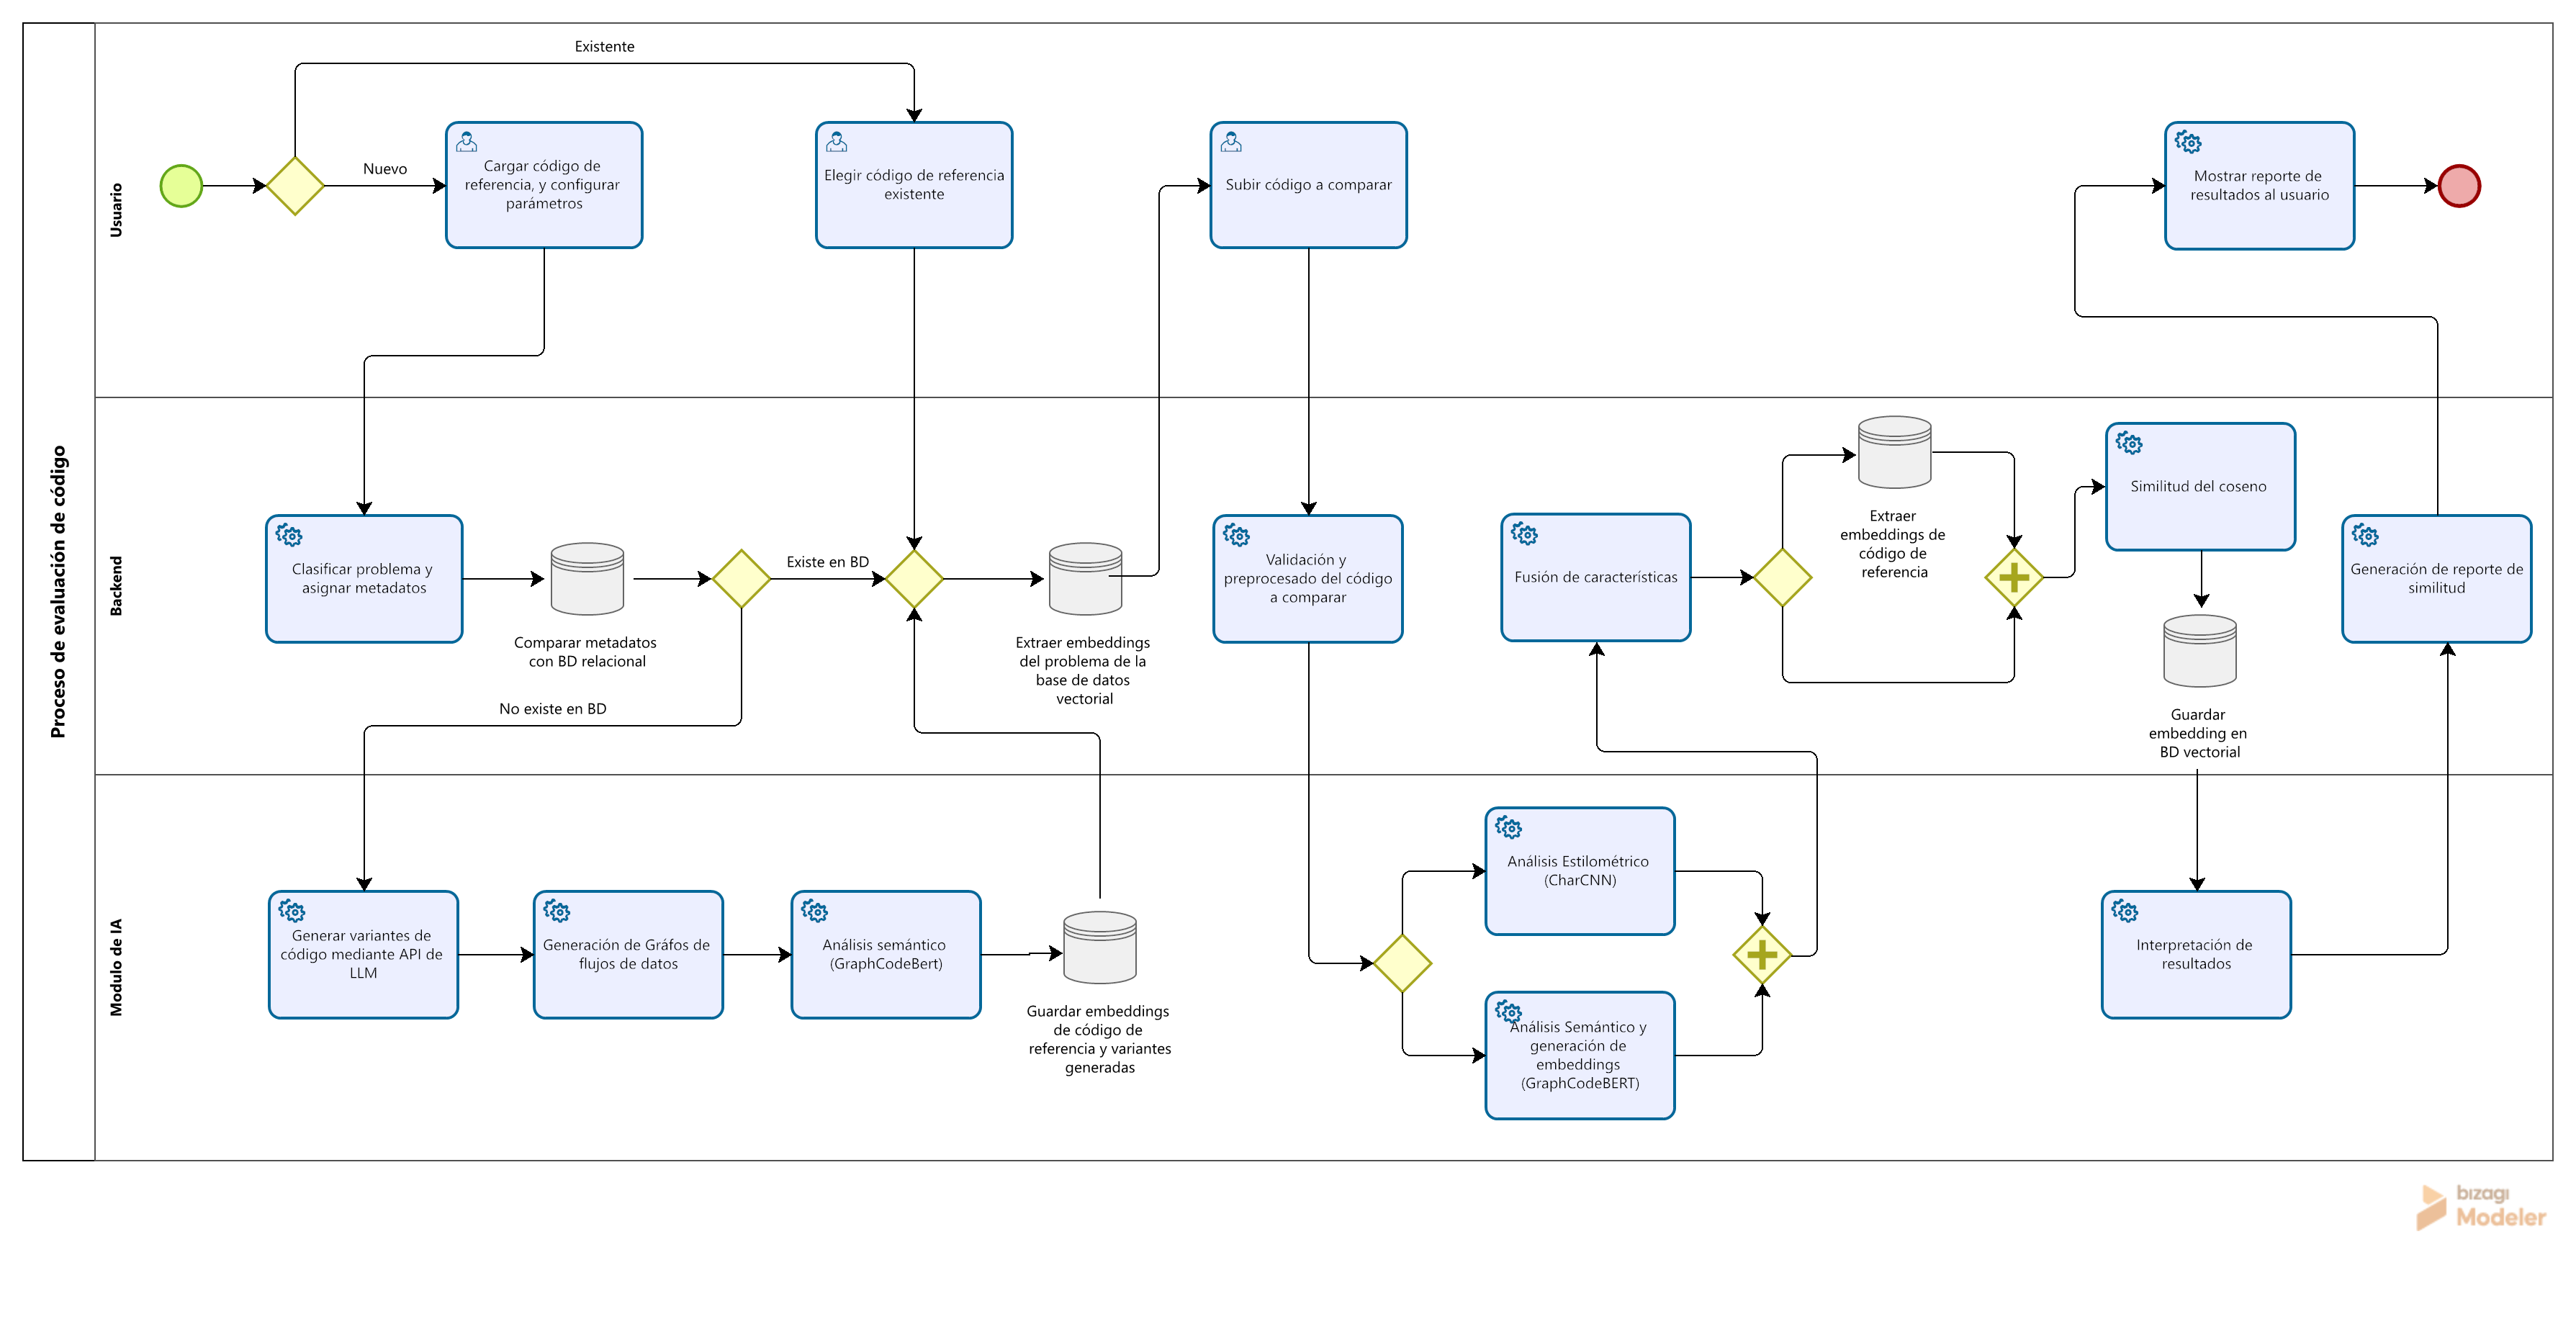
\includegraphics[width=\textwidth]{figuras/ModeloBPMN.png}
    \caption{Diagrama BPMN de la comparación de código fuente.}
    \label{fig:bpmn_proceso}
\end{figure}

% ---------------------------------------------------------
\section{Características semánticas del código}
% ---------------------------------------------------------

A diferencia del análisis estilométrico, el análisis semántico se centra en la lógica subyacente y la funcionalidad del programa, ignorando aspectos superficiales como el nombre de las variables o el formato del texto. Estas características permiten capturar la esencia algorítmica de una solución, lo que facilita la identificación de códigos que, aunque parezcan diferentes visualmente, ejecutan la misma lógica de resolución.

En la Tabla~\ref{tab:caracteristicas_semanticas} se presenta una clasificación de las características semánticas identificadas para la construcción de la firma lógica en este proyecto.

\begin{table}[H]
\centering
\small 
\begin{tabularx}{\textwidth}{l l X}
\toprule
\textbf{Categoría} & \textbf{Característica} & \textbf{Descripción Sintetizada} \\
\midrule
\textbf{Flujo de Datos} & Def-Uso & Rastreo del ciclo de vida y uso de variables. \\
                        & Dependencias & Vínculos lógicos entre variables y operaciones. \\
\midrule
\textbf{Lógica de}      & Caminos & Rutas lógicas y bifurcaciones del algoritmo. \\
\textbf{Control}        & Estructuras & Patrones de repetición y decisiones funcionales. \\
\midrule
\textbf{Representación} & AST / DFG & Jerarquía gramatical y grafo de flujo de datos. \\
\textbf{Estructural}    & Scope & Contexto de validez de las entidades lógicas. \\
\midrule
\textbf{Contexto}       & Semántica & Significado de tokens según su entorno. \\
                        & Equivalencia & Funcionalidad idéntica con distinta sintaxis. \\
\bottomrule
\end{tabularx}
\caption{Clasificación sintetizada de características semánticas del código.}
\label{tab:caracteristicas_semanticas}
\end{table}

La extracción de estas características permite generar una representación robusta ante técnicas de ofuscación comunes, como el renombrado de variables o el cambio de estructuras de control equivalentes (por ejemplo, sustituir un ciclo \textit{for} por un \textit{while}). En este sistema, el uso de \textit{GraphCodeBERT} es fundamental, ya que este modelo no solo procesa el código como una secuencia de texto, sino que incorpora explícitamente el Grafo de Flujo de Datos (DFG). Esto permite que las representaciones vectoriales resultantes capturen de manera profunda las dependencias lógicas, facilitando un análisis semántico preciso incluso cuando la estructura superficial ha sido alterada intencionalmente.

% ---------------------------------------------------------
\section{Características estilométricas del código}
% ---------------------------------------------------------

Para el canal de análisis estilométrico, se identifican diferentes tipos de características que permiten capturar patrones asociados a la escritura del autor. Estas características no dependen de la funcionalidad del programa, sino de la huella digital sintáctica y de formato, lo que permite distinguir entre diferentes autores o identificar probables intervenciones de generación sintética (IA).

En la Tabla~\ref{tab:caracteristicas_estilometricas} se presenta una clasificación de las principales características estilométricas que la red neuronal procesa de forma implícita.

\begin{table}[H]
\centering
\small
\begin{tabular}{lll}
\toprule
\textbf{Categoría} & \textbf{Característica} & \textbf{Descripción} \\
\midrule
Léxicas & Frecuencia de caracteres & Distribución de caracteres y símbolos en el código. \\
        & Uso de palabras clave & Frecuencia de keywords del lenguaje (C11/C++17). \\
        & Longitud de tokens & Tamaño promedio de identificadores y expresiones. \\
\midrule
Sintácticas & Estructuras de control & Preferencia de uso entre if, for, while, switch. \\
            & Anidamiento & Profundidad promedio de los bloques de código. \\
            & Modularidad & Tendencia en la organización en funciones o bloques. \\
\midrule
Formato & Indentación & Uso predominante de espacios o tabulaciones. \\
        & Saltos de línea & Patrones de densidad y distribución de líneas. \\
        & Estilo de llaves & Ubicación de apertura y cierre de bloques \{ \}. \\
\midrule
Estructurales & Tamaño del código & Número total de líneas del archivo original. \\
              & Uso de comentarios & Densidad y ubicación de comentarios respecto al código. \\
\bottomrule
\end{tabular}
\caption{Clasificación de características estilométricas del código fuente.}
\label{tab:caracteristicas_estilometricas}
\end{table}

Estas características permiten construir una representación del estilo de codificación que puede ser utilizada por modelos de aprendizaje automático para identificar anomalías de autoría. En particular, los modelos basados en redes neuronales convolucionales a nivel de caracteres (CharCNN) son capaces de aprender automáticamente patrones locales y distribuciones espaciales en la secuencia de caracteres cruda (preservando el estilo y formato original), lo que resulta especialmente útil para capturar diferencias sutiles entre código escrito por un estudiante humano y código generado de forma automatizada.

% =========================================================
\section{Definición de métricas de desempeño}
% =========================================================

La validación del sistema propuesto requiere la definición de métricas cuantitativas que permitan medir el desempeño algorítmico en los distintos módulos que lo componen. En particular, se consideran los dos componentes de la arquitectura dual: el canal de similitud semántica y el canal de análisis estilométrico.

Cada uno de estos módulos requiere métricas específicas que permitan evaluar su precisión, confiabilidad y utilidad computacional, permitiendo así validar la efectividad de la herramienta como apoyo objetivo a la auditoría docente.

% ---------------------------------------------------------
\subsection{Métricas para el análisis de similitud semántica}
% ---------------------------------------------------------

El canal de análisis semántico tiene como objetivo cuantificar el grado de equivalencia lógica entre dos programas. Para ello, se utilizan representaciones vectoriales (embeddings) generadas mediante el modelo \textit{GraphCodeBERT}.

La principal métrica utilizada es la similitud del coseno, la cual mide el ángulo entre dos vectores en un espacio de alta dimensión. Su valor se encuentra en el rango de [-1, 1], donde valores cercanos a 1 indican una alta proximidad entre los grafos lógicos de los programas analizados.

Esta métrica resulta especialmente adecuada para comparar embeddings, ya que permite determinar la cercanía semántica entre soluciones de software independientemente de su estructura sintáctica superficial.

Adicionalmente, se considera la correlación con el juicio experto como un mecanismo de validación externa, con el fin de determinar si los índices matemáticos generados por el sistema son consistentes con la auditoría manual del evaluador.

% ---------------------------------------------------------
\subsection{Métricas para el análisis estilométrico}
% ---------------------------------------------------------

El canal estilométrico, impulsado por la red neuronal \textit{CharCNN}, se plantea como un problema de clasificación binaria, en el cual se infiere si un fragmento de código presenta patrones de escritura correspondientes a un humano o a generación sintética mediante inteligencia artificial.

Para evaluar el desempeño de este modelo de Deep Learning, se utilizan métricas estándar de clasificación supervisada:

\begin{itemize}
    \item \textbf{Accuracy (Exactitud)}: mide la proporción de predicciones correctas respecto al total de muestras analizadas.
    \item \textbf{Precision (Precisión)}: indica la proporción de predicciones positivas correctas respecto al total de predicciones positivas realizadas.
    \item \textbf{Recall (Exhaustividad)}: mide la capacidad del modelo para identificar correctamente todos los casos positivos reales.
    \item \textbf{F1-score}: representa la media armónica entre precisión y exhaustividad, proporcionando una medida equilibrada del desempeño del modelo ante posibles desbalances de clases.
\end{itemize}

Estas métricas permiten calibrar el comportamiento del modelo en distintos escenarios, particularmente para minimizar la tasa de falsos positivos al detectar anomalías de autoría.

% ---------------------------------------------------------
\subsection{Resumen de métricas utilizadas}
% ---------------------------------------------------------

En la Tabla~\ref{tab:resumen_metricas} se presenta un resumen de las métricas empleadas en cada uno de los módulos de la arquitectura.

\begin{table}[H]
\centering
\begin{tabular}{lll}
\toprule
\textbf{Módulo} & \textbf{Métrica} & \textbf{Propósito} \\
\midrule
Similitud semántica & Similitud del coseno & Medir cercanía espacial entre embeddings. \\
                    & Correlación humana & Validar coherencia con la auditoría docente. \\
\midrule
Análisis estilométrico & Accuracy & Evaluar desempeño general de la red CharCNN. \\
                       & Precision & Medir exactitud en alertas de autoría. \\
                       & Recall & Evaluar detección de anomalías sintéticas. \\
                       & F1-score & Balancear rendimiento ante clases desbalanceadas. \\
\bottomrule
\end{tabular}
\caption{Métricas de validación de modelos utilizadas en el sistema.}
\label{tab:resumen_metricas}
\end{table}

% ---------------------------------------------------------
\subsection{Criterios de interpretación de resultados}
% ---------------------------------------------------------

Para facilitar el análisis de los resultados arrojados por los modelos, se definen criterios de interpretación que permiten contextualizar los valores numéricos obtenidos.

En el caso del canal semántico, los valores de similitud del coseno se interpretan bajo los siguientes umbrales preliminares:

\begin{table}[H]
\centering
\begin{tabular}{ll}
\toprule
\textbf{Rango de similitud} & \textbf{Interpretación algorítmica} \\
\midrule
0.80 -- 1.00 & Alta equivalencia lógica. \\
0.60 -- 0.79 & Equivalencia moderada (posible inspiración estructural). \\
0.40 -- 0.59 & Baja equivalencia. \\
0.00 -- 0.39 & Disimilitud algorítmica. \\
\bottomrule
\end{tabular}
\caption{Criterios de interpretación para similitud semántica espacial.}
\label{tab:criterios_similitud}
\end{table}

Estos rangos permiten identificar casos atípicos y resaltarlos visualmente para revisión detallada del docente, especialmente aquellos que cruzan el umbral de alta equivalencia lógica.

Para el análisis estilométrico, la interpretación técnica se basa en el comportamiento conjunto de las métricas de clasificación:

\begin{itemize}
    \item Valores altos de precisión y exhaustividad indican una sólida capacidad de la CharCNN para diferenciar características de autoría humana versus sintética.
    \item Un F1-score elevado refleja un modelo confiable que no sesga sus clasificaciones hacia la clase mayoritaria.
    \item Diferencias significativas entre precisión y exhaustividad requerirán ajustes en el orquestador para evitar falsos positivos que afecten la transparencia de la auditoría.
\end{itemize}

% ---------------------------------------------------------
\subsection{Consideraciones para la experimentación}
% ---------------------------------------------------------

Para garantizar una validación rigurosa de los modelos, es necesario considerar los siguientes factores durante el diseño del corpus experimental:

\begin{itemize}
    \item \textbf{Diversidad algorítmica}: incluir soluciones con diferentes lógicas de control para el mismo problema.
    \item \textbf{Presencia de variantes IA}: incorporar entregas generadas específicamente mediante la Trayectoria A1 (Modelos de Lenguaje Externos).
    \item \textbf{Balance de clases}: asegurar una distribución representativa entre código escrito por estudiantes y código sintético.
    \item \textbf{Validación cruzada}: aplicar técnicas de partición de datos para evitar el sobreajuste (overfitting) de la red estilométrica.
\end{itemize}

% ---------------------------------------------------------
\subsection{Justificación de las métricas seleccionadas}
% ---------------------------------------------------------

La combinación de estas métricas permite validar el sistema desde dos perspectivas técnicas complementarias. Por un lado, la similitud del coseno aborda el problema de la detección de clones estructurales, cuantificando la equivalencia lógica a través de los grafos. Por otro lado, las métricas de clasificación evalúan la capacidad de la red convolucional para identificar patrones anómalos asociados a la Inteligencia Artificial.

Este enfoque dual permite certificar el desempeño del backend, proporcionando evidencia algorítmica sobre su viabilidad como herramienta de auditoría de código en entornos académicos.

\section{Análisis de riesgos}
% =========================================================

El desarrollo e implementación del sistema propuesto implica la consideración de diversos riesgos que pueden afectar su funcionamiento, desempeño y adopción en el contexto educativo. Estos riesgos pueden surgir tanto a nivel técnico como en el uso práctico del sistema por parte de los evaluadores.

El análisis de riesgos permite identificar posibles escenarios adversos, evaluar su impacto y definir estrategias de mitigación que contribuyan a la robustez, confiabilidad e interpretabilidad del sistema.

% ---------------------------------------------------------
\subsection{Clasificación de riesgos}
% ---------------------------------------------------------

Los riesgos identificados se agrupan en las siguientes categorías:

\begin{itemize}
    \item \textbf{Riesgos técnicos}: relacionados con el funcionamiento de los modelos de inteligencia artificial y la infraestructura del sistema.
    \item \textbf{Riesgos de datos}: asociados a la calidad, disponibilidad y representatividad de los datos utilizados.
    \item \textbf{Riesgos de interpretación}: vinculados a la forma en que los resultados son comprendidos por el evaluador.
    \item \textbf{Riesgos académicos}: relacionados con el impacto del sistema en el proceso de evaluación y aprendizaje.
\end{itemize}

% ---------------------------------------------------------
\subsection{Criterios de evaluación de riesgos}
% ---------------------------------------------------------

Para evaluar los riesgos identificados, se utilizan dos criterios principales: la probabilidad de ocurrencia y el impacto que pueden generar en el sistema.

La \textbf{probabilidad} se refiere a la posibilidad de que un riesgo ocurra durante la operación del sistema, mientras que el \textbf{impacto} describe el nivel de afectación que tendría dicho riesgo en el desempeño, confiabilidad o uso del sistema.

Se consideran tres niveles para cada criterio:

\begin{itemize}
    \item \textbf{Alta}: el riesgo es frecuente o puede afectar significativamente el funcionamiento del sistema.
    \item \textbf{Media}: el riesgo puede ocurrir bajo ciertas condiciones y su impacto es moderado.
    \item \textbf{Baja}: el riesgo es poco probable o su impacto es limitado.
\end{itemize}

Estos niveles permiten priorizar los riesgos y enfocar los esfuerzos de mitigación en aquellos que representan una mayor amenaza para el sistema.

% ---------------------------------------------------------
\subsection{Identificación y evaluación de riesgos}
% ---------------------------------------------------------

En la Tabla X se presentan los principales riesgos identificados, junto con su probabilidad de ocurrencia, impacto y estrategia de mitigación.

\begin{table}[H]
\centering
\begin{tabularx}{\textwidth}{l c c X}
\toprule
\textbf{Riesgo} & \textbf{Prob.} & \textbf{Impacto} & \textbf{Mitigación} \\
\midrule
Baja precisión del modelo semántico & Media & Alta & Ajuste de hiperparámetros y validación con datos reales \\

Clasificación incorrecta en estilometría & Media & Alta & Uso de múltiples métricas y validación cruzada \\

Datos insuficientes o no representativos & Alta & Alta & Ampliación y diversificación del dataset \\

Dependencia de modelos externos (LLM) & Alta & Alta & Uso de rutas de respaldo con modelos alternativos y locales\\

Interpretación incorrecta por el docente & Media & Alta & Visualización clara y explicaciones dentro del sistema \\

Falsos positivos en detección de similitud & Media & Alta & Uso combinado de análisis semántico y estilométrico \\

Alto costo computacional & Media & Media & Optimización del procesamiento y uso de almacenamiento en caché \\

Sesgo en el modelo de clasificación & Media & Alta & Balanceo de clases y evaluación continua del modelo \\

\bottomrule
\end{tabularx}
\caption{Análisis de riesgos del sistema}
\end{table}

% ---------------------------------------------------------
\subsection{Estrategias de mitigación}
% ---------------------------------------------------------

Para reducir el impacto de los riesgos identificados, se plantean diversas estrategias orientadas a mejorar la robustez del sistema:

\begin{itemize}
    \item Validación continua de los modelos mediante conjuntos de datos diversos y representativos.
    \item Integración de múltiples enfoques de análisis (semántico y estilométrico) para reducir errores individuales.
    \item Implementación de mecanismos de interpretación de resultados que faciliten la comprensión por parte del evaluador.
    \item Optimización del rendimiento del sistema para garantizar tiempos de respuesta adecuados.
\end{itemize}

% ---------------------------------------------------------
\subsection{Discusión del impacto de los riesgos}
% ---------------------------------------------------------

El análisis realizado permite identificar que los riesgos con mayor impacto están asociados a la precisión de los modelos de inteligencia artificial y a la interpretación de los resultados en el contexto educativo. Estos factores son críticos, ya que pueden influir directamente en la toma de decisiones del evaluador.

Asimismo, los riesgos relacionados con los datos, como la falta de representatividad o el sesgo, pueden afectar la capacidad del sistema para generalizar correctamente en escenarios reales.

No obstante, mediante la implementación de estrategias de mitigación adecuadas, es posible reducir significativamente estos riesgos, permitiendo que el sistema funcione como una herramienta confiable de apoyo a la evaluación docente.



El análisis de riesgos realizado permite identificar que los factores más críticos del sistema se concentran en la precisión de los modelos de inteligencia artificial y en la correcta interpretación de los resultados por parte del evaluador. Estos elementos son fundamentales, ya que influyen directamente en la confiabilidad del sistema dentro del proceso de evaluación académica.

Asimismo, se observa que los riesgos asociados a la calidad y representatividad de los datos pueden impactar de manera significativa en el desempeño del sistema, particularmente en la capacidad de generalización de los modelos en escenarios reales.

No obstante, la integración de estrategias de mitigación, como el uso combinado de análisis semántico y estilométrico, la validación continua y la incorporación de mecanismos de interpretación, permite reducir estos riesgos y fortalecer la robustez del sistema.

En este sentido, el análisis realizado respalda la viabilidad del sistema propuesto como una herramienta de apoyo a la decisión docente, siempre que se considere como un complemento al criterio humano y no como un sustituto del mismo.


\subsection{Selección y justificación del conjunto de datos}

Para el entrenamiento del clasificador estilométrico propuesto se requieren dos tipos de datos: código fuente escrito por humanos en un contexto educativo introductorio, y código equivalente generado por modelos de inteligencia artificial. A continuación se describe y justifica cada fuente utilizada, así como la estructura cuantitativa del dataset resultante.

\subsubsection{Código humano: IEEE Programming Homework Dataset}

El componente de código humano proviene del \textit{Programming Homework Dataset} publicado por Ljubovic y Pajic (2020) en \cite{Ljubovic2020Dataset}. Este dataset contiene envíos reales de estudiantes en dos cursos introductorios de programación universitaria: el curso A en lenguaje C y el curso B en C++, con entre 16 y 22 asignaciones por curso. Su selección se justifica por tres razones principales.

En primer lugar, el origen de los datos es directamente relevante al dominio del problema. Los envíos provienen de estudiantes en cursos de fundamentos de programación, que es exactamente la población objetivo del sistema propuesto. Esto garantiza que el modelo aprenda patrones estilométricos propios del código estudiantil introductorio y no de programadores expertos o código de producción.

En segundo lugar, el dataset cubre los tipos de problemas de interés: estructuras de control, manejo de arreglos, funciones, estructuras de datos básicas y manejo de archivos, todos representativos del currículo de un curso introductorio de C/C++ (acorde a los estándares C11 y C++17).

En tercer lugar, respecto al idioma de los identificadores y comentarios, el análisis del código fuente contenido en el dataset confirmó que este se encuentra escrito en serbocroata con alfabeto latino. Dado que los comentarios constituyen un rasgo estilométrico relevante —puesto que codifican información sobre la frecuencia, extensión y estilo de documentación del programador—, estos se conservan íntegramente durante el preprocesamiento como parte del \textit{input} de la CharCNN. La compatibilidad general con código escrito en otros idiomas de alfabeto latino, como el español o el inglés, se garantiza a nivel de distribución de caracteres y topología estructural.

\subsubsection{Código generado por IA (Clase Sintética)}

Para construir la clase positiva del clasificador (código generado por IA), se opta por una estrategia de generación propia sobre los mismos enunciados de problemas presentes en el dataset humano. Esta decisión se fundamenta en la necesidad de que ambas clases respondan al mismo dominio del problema, evitando que el modelo aprenda diferencias asociadas a la lógica de la tarea y no a la naturaleza de su origen (humano vs. máquina).

Con el objetivo de maximizar la generalización de la red convolucional ante distintos modelos de lenguaje, se emplea un conjunto diverso de generadores organizado en dos niveles, como se resume en la Tabla \ref{tab:composicion_dataset}. En el primer nivel se incluyen modelos de referencia comerciales (SOTA), mientras que el segundo nivel abarca modelos de código abierto.

\begin{table}[ht]
\centering
\caption{Composición y origen del conjunto de datos dual}
\label{tab:composicion_dataset}
\renewcommand{\arraystretch}{1.6}
\begin{tabularx}{\textwidth}{>{\raggedright\arraybackslash}p{2.5cm} >{\raggedright\arraybackslash}p{2.5cm} >{\raggedright\arraybackslash}p{1.5cm} >{\raggedright\arraybackslash}p{2.5cm} >{\raggedright\arraybackslash}X}
\toprule
\textbf{Categoría} & \textbf{Fuente / Modelo} & \textbf{Lenguaje} & \textbf{Origen de Escritura} & \textbf{Propósito en el sistema} \\
\midrule
Código Humano & IEEE Programming Homework \cite{Ljubovic2020Dataset} & C / C++ & Estudiante (Humano) & Base de referencia de escritura manual y entrenamiento de CharCNN. \\

\addlinespace

Código IA (Comercial) & GPT-4o, Claude 3.5, Gemini 1.5 & C / C++ & Generativo (SOTA) & Identificación de patrones de IAs de alta disponibilidad para estudiantes. \\

\addlinespace

Código IA (Local) & CodeLlama, DeepSeek, Qwen2.5 & C / C++ & Generativo (Open-Source) & Evaluación de robustez ante modelos locales y diversidad estilística. \\
\bottomrule
\end{tabularx}
\smallskip
\footnotesize\textit{Elaboración propia con base en \cite{Ljubovic2020Dataset}.}
\end{table}

Para garantizar la consistencia entre ambas clases, todos los \textit{prompts} de generación se formulan indicando explícitamente al modelo que utilice nombres de variables y comentarios en serbocroata. Esto asegura que el idioma no constituya una señal discriminante (sesgo) durante el entrenamiento, forzando a la red a aprender diferencias estrictamente de naturaleza estilométrica espacial. Adicionalmente, se generan variantes de \textit{prompt} para cada problema con el fin de reducir la dependencia a un estilo de generación único:

\begin{itemize}
    \item Un \textit{prompt} directo con el enunciado del problema.
    \item Un \textit{prompt} con instrucción de simular el estilo de un estudiante principiante.
    \item Un \textit{prompt} con enfoque en optimización sin instrucciones de estilo adicionales.
\end{itemize}

\subsubsection{Consideraciones de balance y partición}

El corpus final se construye con clases estrictamente balanceadas (50\% humano, 50\% IA) para evitar sesgos de clase mayoritaria en las predicciones de la CharCNN. La partición de los datos se realiza a nivel de \textit{problema}; es decir, todas las soluciones (humanas o sintéticas) de un problema específico aparecen exclusivamente en una de las fases (entrenamiento, validación o prueba). Esta restricción arquitectónica previene la fuga de información (\textit{data leakage}), obligando al modelo a clasificar basándose en el estilo y no en la lógica del algoritmo. La Tabla \ref{tab:distribucion_muestras} presenta la distribución cuantitativa establecida.

\begin{table}[ht]
\centering
\caption{Distribución cuantitativa y partición del conjunto de datos}
\label{tab:distribucion_muestras}
\renewcommand{\arraystretch}{1.6}
\begin{tabularx}{\textwidth}{l c c X}
\toprule
\textbf{Subconjunto} & \textbf{Porcentaje} & \textbf{Cantidad ($n$)} & \textbf{Finalidad en el modelo} \\
\midrule
Entrenamiento (\textit{Train}) & 70\% & 14,000 & Ajuste de pesos y aprendizaje de características estilométricas 1D. \\

\addlinespace

Validación (\textit{Val}) & 15\% & 3,000 & Ajuste de hiperparámetros y prevención de \textit{overfitting} durante el entrenamiento. \\

\addlinespace

Prueba (\textit{Test}) & 15\% & 3,000 & Evaluación cuantitativa del rendimiento y matriz de confusión en datos no vistos. \\

\midrule
\textbf{Total ($N$)} & \textbf{100\%} & \textbf{20,000} & \textbf{Dataset consolidado e híbrido.} \\
\bottomrule
\end{tabularx}
\smallskip
\footnotesize\textit{Elaboración propia.}
\end{table}

En conclusión, la estructuración de este corpus híbrido permite calibrar con precisión el canal estilométrico del sistema \textbf{Graphito}. El diseño metodológico empleado fuerza a la arquitectura CharCNN a desarrollar una alta sensibilidad a las micro-estructuras de estilo que diferencian el código orgánico del sintético. El uso de $N = 20,000$ muestras asegura una base estadística robusta para generalizar características más allá de las palabras clave, capturando la huella digital del código fuente en entornos académicos iniciales.